%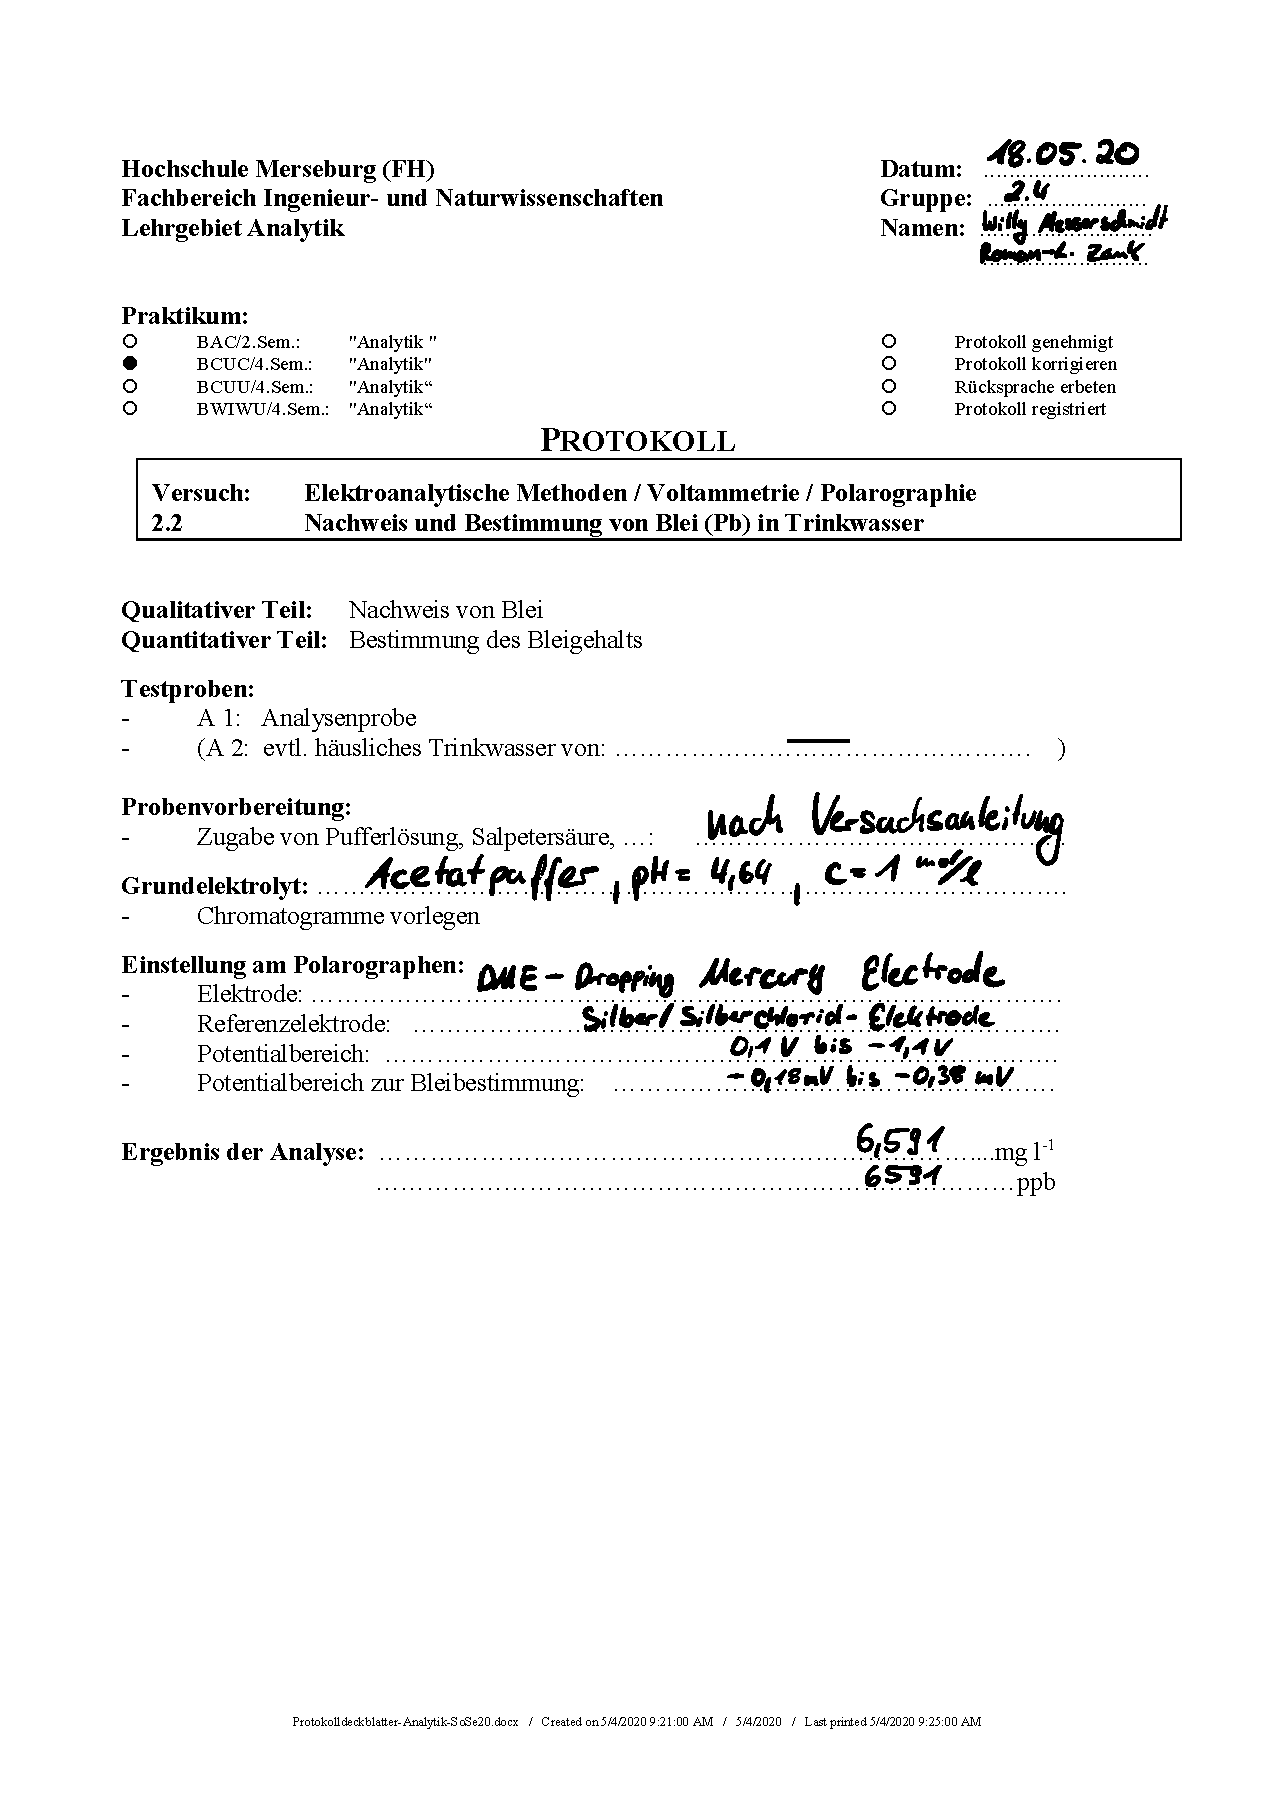
\includepdf[]{Deckblatt}
\pagebreak
\section{Einleitung}
\label{sec:einleitung}
In diesem Versuch soll Ammonium in verschiedenen Wasserproben, mittels Photometrie, quantifiziert werden. Da Ammonium ein wesentlicher Bestandteil des Stickstoffkreislaufes in Ökosystemen dargestellt, ist die Betrachtung des Ammonium-Gehaltes in Gewässern von großer Bedeutung. Abwässer, sowie Düngerausschwemmungen oder der Abbau von Extrementen können als Quelle für Ammonium-Ionen in Böden und Gewässern fungieren. Gerade proteinreiche, organische Substanzen stehen dabei im Fokus \mbox{(siehe Gl. \eqref{gl:1})}. Dabei entziehen die Ammonium-Ionen, durch den Prozess der Nitrifikation \mbox{(siehe Gl. \eqref{gl:2})}, Sauerstoff. Dieser ist für Wasserorganismen lebenswichtig. Daraus ergibt sich, dass Wässer wie unbelastete Oberflächengewässer, Kläranlagenabläufe oder Trinkwasser gewisse Grenzwerte einzuhalten haben.\\
Diese Grenzwerte werden für der zur Verfügung gestellten Proben untersucht.\\ \\
\textbf{Prozess der Ammonifikation:}
\begin{flalign}
	\label{gl:1}
	\ce{R-NH2 + H2O &-> NH3 + R-OH}\\
	\ce{NH3 &->[H2O] NH4+}
\end{flalign}

\textbf{Prozess der Nitrifikation:}
\begin{flalign}
	\label{gl:2}
	\ce{2 NH3 + 3 O2 &-> 2 NO2- + 2 H+ + 2 H2O}\\
	\ce{2 NO2- + O2 &-> 2 NO3-}
\end{flalign}







